%==============================================================================
%  FamilyFinanceChat -- Fall 2026 Project Overview -- BUILD-STEP EDITION
%
%  Same 10 slides as familyfinancechat-fall2026.tex, but each slide is broken
%  into CUMULATIVE overlay steps: one PDF page per revealed element.  Each page
%  becomes one PowerPoint slide, so the narration in the speaker notes stays
%  synchronised with whatever has just appeared on screen.
%
%  This file exists for the HeyGen video.  The 10-slide file remains the deck
%  for a live human presenter -- keep the two in sync by hand if either changes.
%
%  Every frame fixes its own bounding box (\useasboundingbox, \onslide rather
%  than \only, \item<n-> rather than \item<only@n>) so that nothing shifts
%  position between build steps.  A moving layout looks like a glitch on video.
%
%  Build:  ./build.sh video        (or: latexmk -pdf familyfinancechat-fall2026-build.tex)
%  Then:   python3 build-heygen-pptx.py
%==============================================================================
\documentclass[aspectratio=169,11pt]{beamer}

\usepackage[T1]{fontenc}
\usepackage[utf8]{inputenc}
\usepackage{helvet}
\renewcommand{\familydefault}{\sfdefault}
\usepackage{microtype}
\usepackage{tikz}
\usepackage{xcolor}
\usetikzlibrary{arrows.meta,positioning,fit,backgrounds}

%------------------------------------------------------------------ palette --
\definecolor{ffcInk}{HTML}{16213A}
\definecolor{ffcBlue}{HTML}{1F4E8C}
\definecolor{ffcTeal}{HTML}{147D82}
\definecolor{ffcRed}{HTML}{A32A2A}
\definecolor{ffcGrey}{HTML}{5A6472}
\definecolor{ffcMist}{HTML}{EEF1F6}
\definecolor{ffcRule}{HTML}{C9D2E0}

%--------------------------------------------------------------------- theme --
\usetheme{default}
\usecolortheme{default}
\setbeamercolor{normal text}{fg=ffcInk}
\setbeamercolor{structure}{fg=ffcBlue}
\setbeamercolor{frametitle}{fg=white,bg=ffcInk}
\setbeamerfont{frametitle}{series=\bfseries,size=\large}
\setbeamertemplate{navigation symbols}{}
\setbeamertemplate{itemize item}{\color{ffcBlue}\rule[0.35ex]{0.7ex}{0.7ex}}
% Uncovered-but-not-yet-shown material is fully transparent, not greyed out:
% a ghosted preview of the next bullet is a distraction on video.
\setbeamercovered{invisible}

\setbeamertemplate{frametitle}{%
  \nointerlineskip
  \begin{beamercolorbox}[wd=\paperwidth,ht=3.1ex,dp=1.5ex,leftskip=0.9em,rightskip=0.9em]{frametitle}
    \usebeamerfont{frametitle}\insertframetitle%
    \hfill\raisebox{0.2ex}{\scriptsize\color{ffcRule}\insertframenumber}
  \end{beamercolorbox}%
  \vskip1.2ex
}
\setbeamertemplate{footline}{%
  \hbox{\begin{beamercolorbox}[wd=\paperwidth,ht=2.2ex,dp=1ex,leftskip=0.9em,rightskip=0.9em]{}
    {\tiny\color{ffcGrey}FamilyFinanceChat \quad$\cdot$\quad Fall 2026}
  \end{beamercolorbox}}
}

%----------------------------------------------------------------- shortcuts --
\newcommand{\hl}[1]{\textcolor{ffcBlue}{\textbf{#1}}}
\newcommand{\bad}[1]{\textcolor{ffcRed}{\textbf{#1}}}
\newcommand{\good}[1]{\textcolor{ffcTeal}{\textbf{#1}}}

\newcommand{\point}[2]{%
  \noindent\begin{minipage}{\textwidth}
    {\color{ffcBlue}\large\bfseries #1}\quad{\large #2}
  \end{minipage}\\[1.0em]}

\tikzset{
  box/.style={rounded corners=3pt,draw=ffcRule,fill=white,inner sep=8pt,
              align=center,font=\small,minimum height=13mm,minimum width=28mm},
  core/.style={box,fill=ffcMist,draw=ffcBlue,font=\small\bfseries},
  newb/.style={box,fill=ffcTeal!14,draw=ffcTeal,font=\small\bfseries},
  arr/.style={-{Stealth[length=6pt]},draw=ffcGrey,semithick},
  lbl/.style={font=\scriptsize,text=ffcGrey,inner sep=3pt},
}

\begin{document}

%== 1 == Title ============================================== 2 steps ========
\begin{frame}[plain]
  \begin{tikzpicture}[remember picture,overlay]
    \fill[ffcInk] (current page.south west) rectangle (current page.north east);
    \fill[ffcTeal] ([xshift=1.3cm,yshift=1.45cm]current page.west) rectangle
                   ([xshift=2.9cm,yshift=1.56cm]current page.west);
    \node[anchor=west,text width=0.82\paperwidth] at ([xshift=1.3cm,yshift=0.6cm]current page.west)
      {\color{white}\Huge\bfseries FamilyFinanceChat};
    \node<2->[anchor=west,text width=0.82\paperwidth] at ([xshift=1.3cm,yshift=-0.8cm]current page.west)
      {\color{ffcRule}\LARGE Fall 2026: make it solid, give it a face};
    \node<1->[anchor=west,text width=0.82\paperwidth] at ([xshift=1.3cm,yshift=-2.2cm]current page.west)
      {\color{white}\small\bfseries Professor Mark Fedenia\hspace{0.5em}%
       \color{ffcGrey}\mdseries directing the project};
    \node<1->[anchor=west,text width=0.82\paperwidth] at ([xshift=1.3cm,yshift=-3.0cm]current page.west)
      {\color{ffcGrey}\footnotesize FIN 602 Capstone Engineering Team};
    \node<1->[anchor=west,text width=0.82\paperwidth] at ([xshift=1.3cm,yshift=-3.55cm]current page.west)
      {\color{ffcGrey}\footnotesize For a spring class in Wealth Management \& Financial Planning};
  \end{tikzpicture}
\end{frame}

%== 2 == What we have ======================================= 3 steps ========
\begin{frame}{What we have}
  \vfill
  \begin{center}
  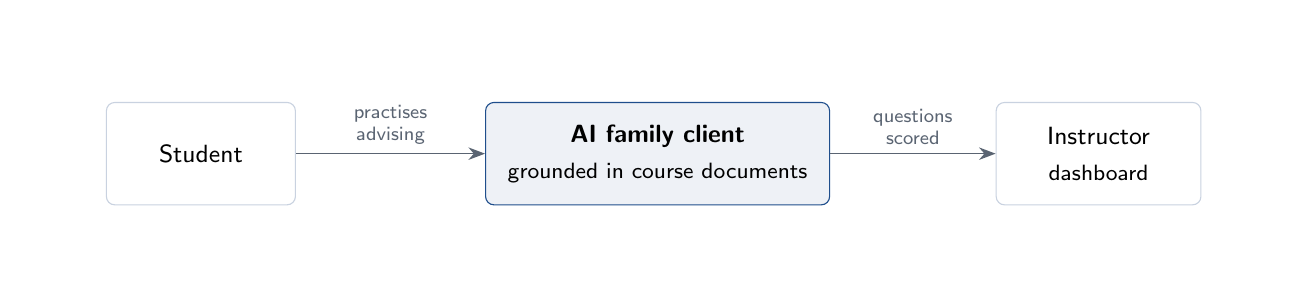
\begin{tikzpicture}
    \useasboundingbox (-2.2,-1.6) rectangle (13.6,1.6);
    \node<1->[box,minimum width=24mm] at (0,0) (stu) {Student};
    \node<1->[core,minimum width=38mm] at (5.8,0) (ow)
      {AI family client\\[2pt] {\footnotesize\mdseries grounded in course documents}};
    \node<2->[box,minimum width=26mm] at (11.4,0) (ins) {Instructor\\[2pt] {\footnotesize\mdseries dashboard}};
    \draw<1->[arr] (stu) -- node[lbl,above,align=center]{practises\\advising} (ow);
    \draw<2->[arr] (ow) -- node[lbl,above,align=center]{questions\\scored} (ins);
  \end{tikzpicture}
  \end{center}
  \vfill
  \begin{center}\large
  \onslide<3->{Unlimited practice, at any hour, without booking a human role-player.}
  \end{center}
  \vfill
\end{frame}

%== 3 == Three things hurt ================================== 4 steps ========
\begin{frame}{It works. Three things hurt.}
  \vspace{1.4em}
  \onslide<1->{\point{1}{We are \bad{three versions behind} the software we run on.}}
  \onslide<2->{\point{2}{The professor's grading tool \bad{runs on a laptop}, not a website.}}
  \onslide<3->{\point{3}{Every deployment needs \bad{manual steps} that people forget.}}
  \vfill
  \begin{center}\large
  \onslide<4->{The gap between \emph{a system that works} and \emph{a system you can hand over}.}
  \end{center}
  \vspace{1.0em}
\end{frame}

%== 4 == The one rule ======================================= 3 steps ========
\begin{frame}{The one rule}
  \vfill
  \begin{center}
    {\Huge\bfseries\color{ffcBlue} Never modify Open WebUI's core.}
  \end{center}
  \vfill
  \begin{center}
  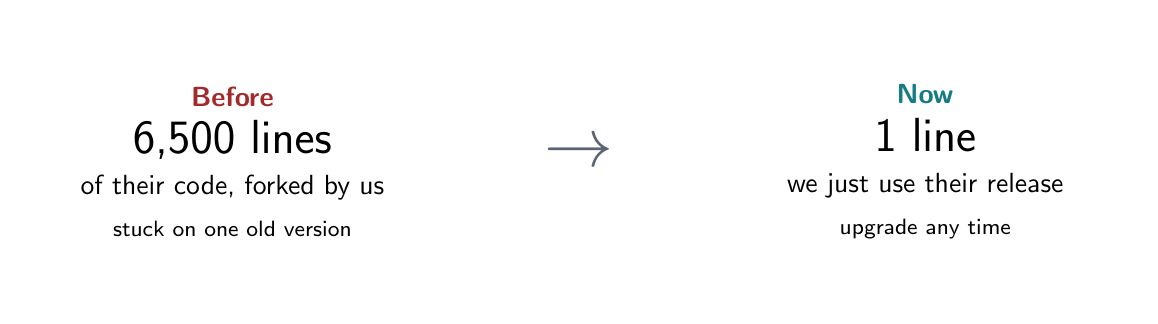
\begin{tikzpicture}
    \useasboundingbox (-2.6,-1.7) rectangle (11.4,1.7);
    \node<2->[align=center,font=\normalsize] at (0,0)
      {\bad{Before}\\[5pt] {\LARGE 6{,}500 lines}\\[3pt] of their code, forked by us\\[3pt]
       {\footnotesize stuck on one old version}};
    \node<2->[font=\Huge,text=ffcGrey] at (4.4,0.1) {$\rightarrow$};
    \node<2->[align=center,font=\normalsize] at (8.8,0)
      {\good{Now}\\[5pt] {\LARGE 1 line}\\[3pt] we just use their release\\[3pt]
       {\footnotesize upgrade any time}};
  \end{tikzpicture}
  \end{center}
  \vfill
  \begin{center}\large
  \onslide<3->{The test: \emph{could we take their next release tomorrow, unchanged?}}
  \end{center}
  \vfill
\end{frame}

%== 5 == Workstream A ======================================= 4 steps ========
\begin{frame}{First job: make it solid}
  \vspace{1.6em}
  \begin{center}
  \begin{minipage}{0.86\textwidth}\large
    \begin{itemize}\setlength{\itemsep}{0.95em}
      \item<1-> Upgrade to the \hl{current version} --- carefully, one step at a time
      \item<2-> Give the professor a \hl{web address} instead of a laptop
      \item<3-> \hl{Automate} deployment and testing, so upgrades stop breaking things quietly
      \item<4-> \hl{Delete} the last remnants of the old fork
    \end{itemize}
  \end{minipage}
  \end{center}
  \vfill
\end{frame}

%== 6 == Workstream B ======================================= 3 steps ========
\begin{frame}{Second job: give the client a face}
  \vfill
  \begin{center}
    {\Large Today the student \emph{types} to the client.}\\[1.3em]
    {\Huge\bfseries\color{ffcTeal} \onslide<2->{We want them to talk to it.}}\\[1.3em]
    {\Large \onslide<2->{A face that listens, and answers out loud.}}
  \end{center}
  \vfill
  \begin{center}\large
  \onslide<3->{You cannot rehearse a hard question about money\\[0.2em] when you have a backspace key.}
  \end{center}
  \vfill
\end{frame}

%== 7 == How, without breaking the rule ===================== 4 steps ========
\begin{frame}{How --- without breaking the rule}
  \vfill
  \begin{center}
  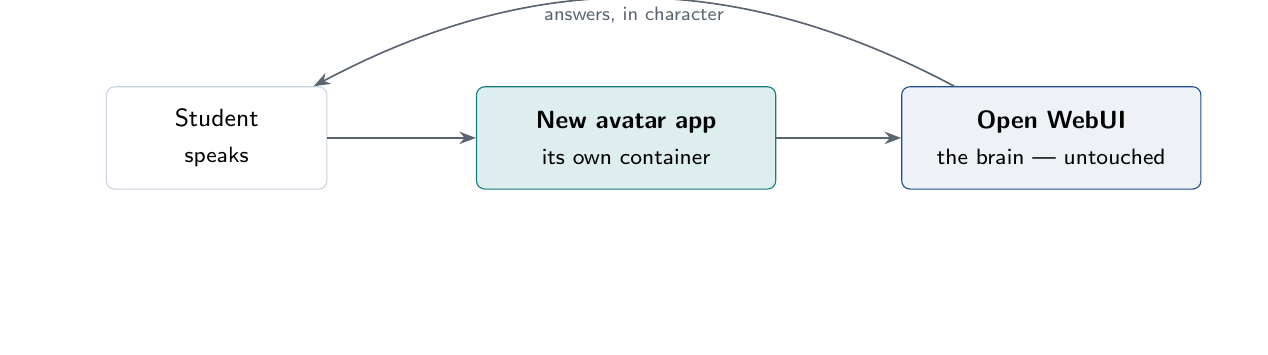
\begin{tikzpicture}
    \useasboundingbox (-2.4,-2.4) rectangle (13.0,1.4);
    \node<1->[box] at (0,0) (stu) {Student\\[2pt] {\footnotesize\mdseries speaks}};
    \node<2->[newb,minimum width=38mm] at (5.2,0) (app) {New avatar app\\[2pt] {\footnotesize\mdseries its own container}};
    \node<3->[core,minimum width=38mm] at (10.6,0) (ow) {Open WebUI\\[2pt] {\footnotesize\mdseries the brain --- untouched}};
    \draw<2->[arr] (stu) -- (app);
    \draw<3->[arr] (app) -- (ow);
    \draw<3->[arr] (ow) to[bend right=28] node[lbl,below]{answers, in character} (stu);
  \end{tikzpicture}
  \end{center}
  \vfill
  \begin{center}\large
  \onslide<2->{A \hl{separate app} beside the platform --- never inside it.}
  \end{center}
  \vspace{0.5em}
  \begin{center}\normalsize
  \onslide<4->{If it does not work out, we delete one container. Nothing to unpick.}
  \end{center}
  \vfill
\end{frame}

%== 8 == Three numbers ====================================== 4 steps ========
\begin{frame}{Three numbers decide whether it works}
  \vspace{2.0em}
  \begin{columns}[T,onlytextwidth]
    \begin{column}{0.31\textwidth}
      \onslide<1->{\begin{center}
        {\Huge\bfseries\color{ffcBlue} 1.2\,s}\\[0.8em]
        {\large to answer}\\[0.5em]
        {\footnotesize Slower than that and it stops feeling like a conversation.}
      \end{center}}
    \end{column}
    \begin{column}{0.31\textwidth}
      \onslide<2->{\begin{center}
        {\Huge\bfseries\color{ffcBlue} \$400}\\[0.8em]
        {\large per semester}\\[0.5em]
        {\footnotesize Roughly, for a class of forty. Capped, so it cannot run away.}
      \end{center}}
    \end{column}
    \begin{column}{0.31\textwidth}
      \onslide<3->{\begin{center}
        {\Huge\bfseries\color{ffcBlue} Week 2}\\[0.8em]
        {\large consent settled}\\[0.5em]
        {\footnotesize Voice and video are student records. Agreed before anything is recorded.}
      \end{center}}
    \end{column}
  \end{columns}
  \vfill
  \begin{center}\large
  \onslide<4->{If any one of them fails, the answer is \bad{no} --- and no is an acceptable answer.}
  \end{center}
  \vspace{0.8em}
\end{frame}

%== 9 == The semester ======================================= 5 steps ========
\begin{frame}{The semester}
  \vspace{1.6em}
  \begin{center}
  \begin{minipage}{0.90\textwidth}\large
    \begin{itemize}\setlength{\itemsep}{0.9em}
      \item<1->[\textbf{\color{ffcBlue}29 Sep}] Students can \hl{talk to it} --- voice only, no face yet
      \item<2->[\textbf{\color{ffcBlue}20 Oct}] Pick an avatar provider --- \hl{or decide to stop}
      \item<3->[\textbf{\color{ffcBlue}27 Oct}] Platform \hl{upgraded} and running current
      \item<4->[\textbf{\color{ffcBlue}17 Nov}] Five students complete \hl{full spoken sessions}, graded normally
    \end{itemize}
  \end{minipage}
  \end{center}
  \vfill
  \begin{center}\normalsize
  \onslide<5->{Weekly check-in every Tuesday, 15 September to 1 December.\\[0.3em]
  Voice-only ships in September either way. \emph{The avatar is allowed to fail.}}
  \end{center}
  \vspace{0.8em}
\end{frame}

%== 10 == Done / close ====================================== 4 steps ========
\begin{frame}{What finished looks like}
  \vspace{1.2em}
  \begin{center}
  \begin{minipage}{0.88\textwidth}\large
    \begin{itemize}\setlength{\itemsep}{0.8em}
      \item<1-> A professor grades from \hl{a web address} --- no laptop
      \item<2-> Deployments are \hl{automatic}; bad changes never ship
      \item<3-> We know, \hl{with evidence}, whether the avatar helps
    \end{itemize}
  \end{minipage}
  \end{center}
  \vspace{2.4em}
  \begin{center}
    \onslide<4->{{\Large The goal is not to finish this system.}\\[0.6em]
    {\Large It is to leave one where the interesting work is}\\[0.4em]
    {\Large\bfseries\color{ffcBlue} the teaching, not the plumbing.}}
  \end{center}
  \vfill
\end{frame}

\end{document}
